\subsection{Motivation for Morse theory}

\subsection{Handle Decompositions}
What is a handle? Let us fix a little notation for the rest this section. A manifold $M$ will be a compact manifold with boundary $\partial M$. We will say a manifold is \textbf{closed} if $\partial M = \varnothing$. We will denote the closed k-ball as follows:
\[
D^{k}= \{ x \in \RR^{k} \big| ~|x| \leq 1 \}.
\]
Further, all maps between manifolds will be assumed smooth ($C^{\infty}$) unless explicitly stated.
\begin{definition}
Let $M$ be an n-dimensional manifold. Let $0\leq k \leq n$. Then an n-dimensional \textbf{k - handle} is the set $D^{k} \times D^{n-k}$, together with an embedding 
\[
\phi : \partial D^{k}\times D^{n-k} \rightarrow \partial M
\]
\end{definition}
The thing to remember is that handles get attached. The quotient space $M \sqcup D^{k}\times D^{n-k} /_{x\sim \phi(x)}$ is the result of attaching a k-handle.

There are some parts of a handle with which we would like to keep track of. There is the \textbf{attaching region}, $\partial D^{k} \times D^{n-k}$, which we discussed above. There is the \textbf{core} of the handle, $D^{k}\times \{0\}$. Associated with the core is the \textbf{attaching sphere} $\partial D^{k} \times \{0\}$. Lastly, we have the \textbf{cocore}, $\{0\}\times D^{n-k}$ and the \textbf{belt sphere}, $\{0\}\times \partial D^{n-k}$.
\begin{example} Let k = 1, n = 3, and let $M$ be $D^{3}$. Thus our handle is a copy of $D^{1}\times D^{2}$ together with an embedding $\phi: S^{0}\times D^{2} \rightarrow S^{2}$.
\begin{figure}[h]
    \centering
    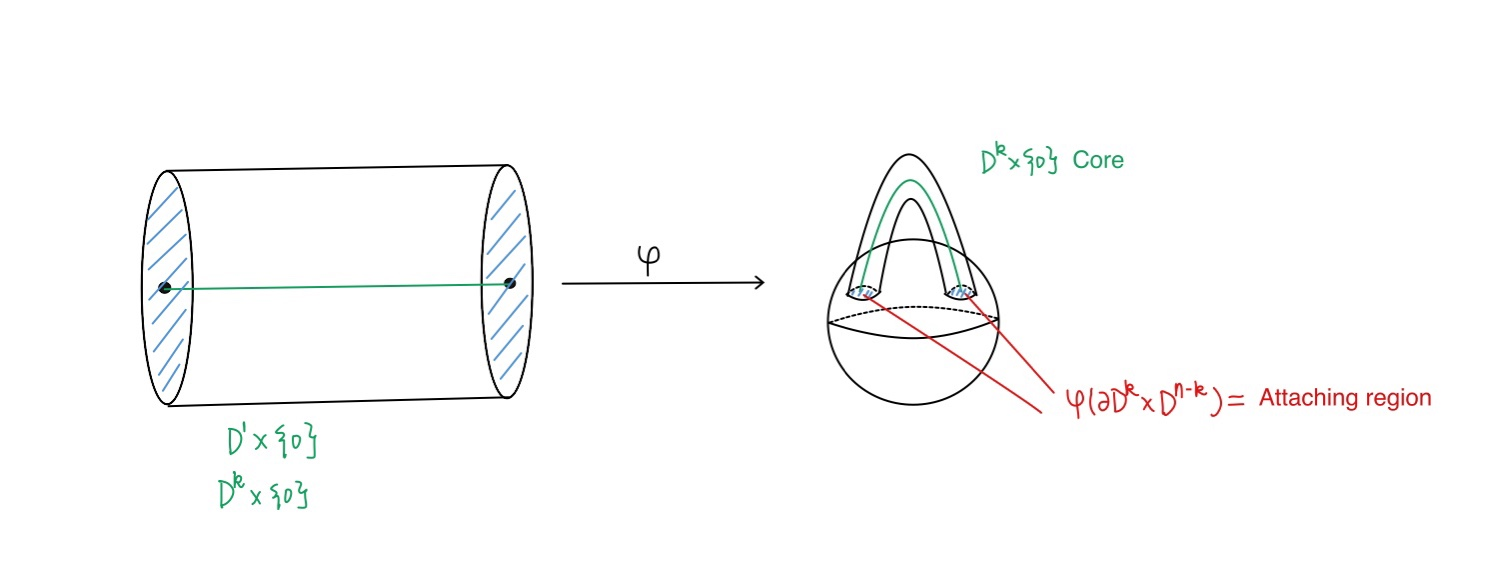
\includegraphics[width = .8\linewidth]{Images_Lect1/3-dimensional_1-handle.jpeg}
    \caption{Attaching a 1 handle}
    \label{fig:1handle}
\end{figure}
\end{example}
\begin{example}
Let k = 0, n = 3 \footnote{we will let $n \leq 3$ most of the time so that we can draw pictures.}. Then a 0 handle is just $\{0 \} \times D^{3} \simeq D^{3}$. The attaching region is empty! So attaching the 0 handle is just taking the disjoint union with $D^{3}$.
\begin{figure}[h!]
    \centering
    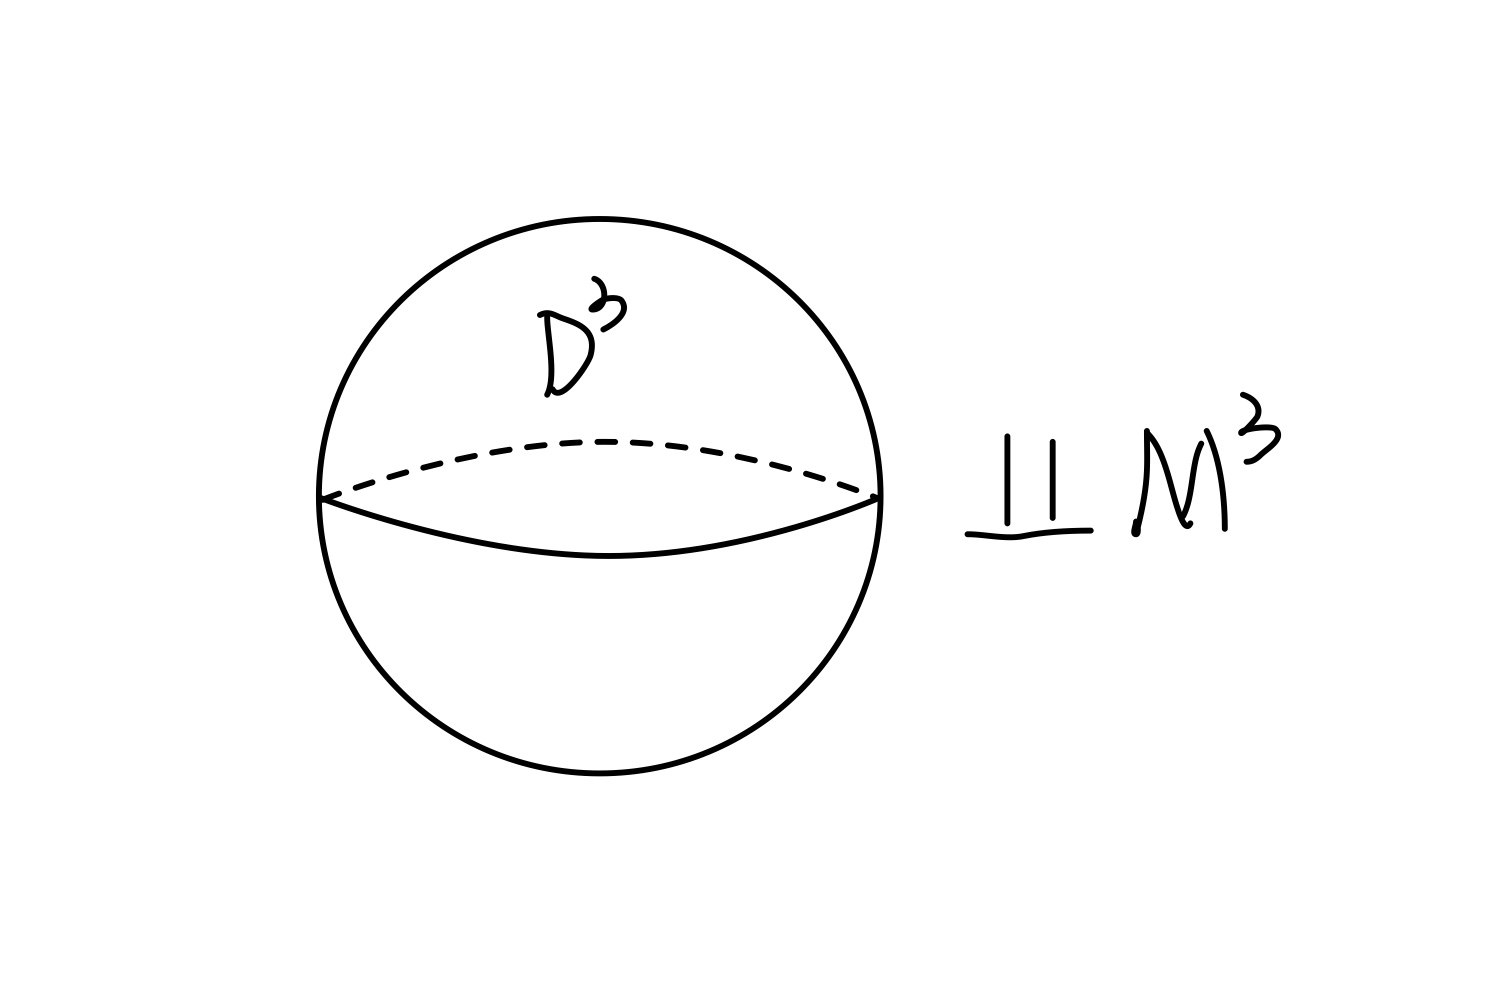
\includegraphics[width = .3\linewidth]{Images_Lect1/0handle.jpeg}
    \caption{Attaching a 1 handle}
    \label{fig:0handle}
\end{figure}
\end{example}
\begin{example}
Lets consider $S^{2}$. Now if we separate the top half and bottom half of $S^{2}$ at the equator, then we have decomposed $S^{2}$ into two pieces which are glued together along their boundaries.

Examining this example a little more carefully, if we imagine $S^{2}\subset \RR^{3}$, given by the standard embedding,
\[
\{(x,y,z) \big| ~ x^{2}+y^{2}+z^{2}=1\}
\]
together with the projection map, $\pi(x,y,z) = z$, restricted to $S^{2}$, we can consider what happens as we let $z$ move from $-\infty$ to $\infty$. While $z< -1$, $\pi^{-1}(z) = \varnothing$. Then, once z crosses $-1$, $\pi^{-1}((-\infty, z]) \simeq D^{2}$. What happened? We attached a 0-cell. Thus crossing -1 corresponds to attaching a 0-cell to $\varnothing$. Continuing on, nothing changes until we cross the point $z=1$. What happens there? We attach a 2 -cell. 
\end{example}

\begin{figure}[h]
    \centering
    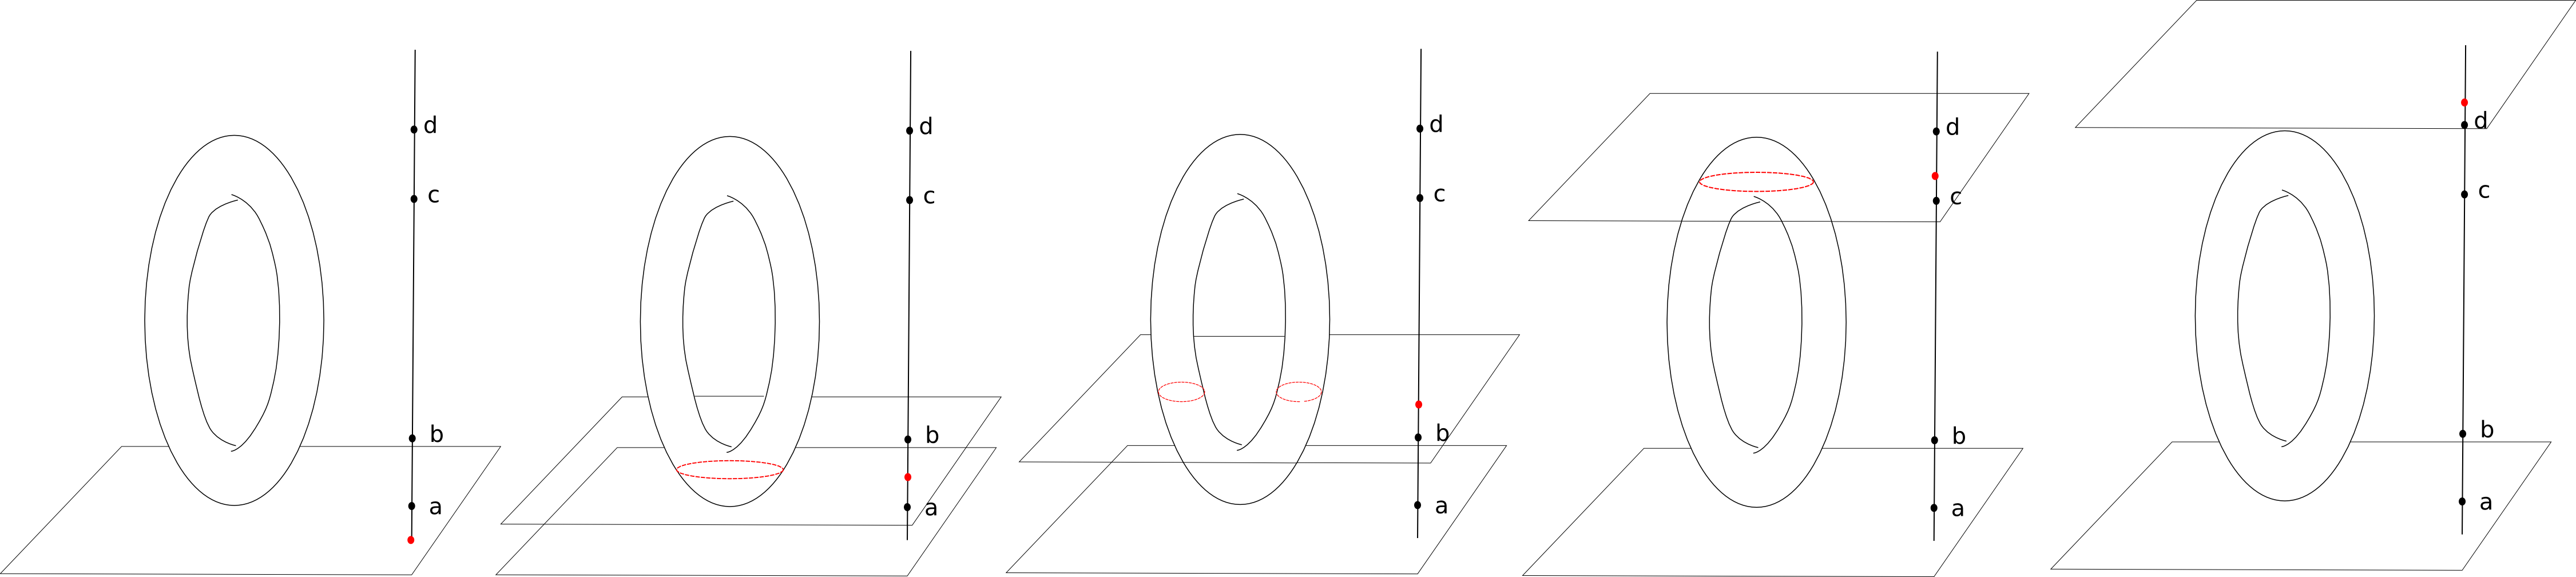
\includegraphics[width = .8\linewidth]{Images_Lect1/image.png}
    \caption{Torus with a height function}
    \label{fig:Torus}
\end{figure}
\begin{example}
Lets consider the embedding of $T^{2}= S^{1}\times S^{1}$ in $\RR^{3}$ as shown in Figure \ref{fig:Torus}. Again we will consider the projection onto the z axis, $\pi$, restricted to $T^{2}$, along with $\phi$, the projection onto the x-y plane. 

I have labeled 4 points on the z axis in the figure. Just like in the case of the 2 sphere, when $z < a$, there is nothing in the preimage of $\pi$, and crossing $a$, we attach a 0- cell to $\varnothing$.
\begin{figure}[h]
    \centering
    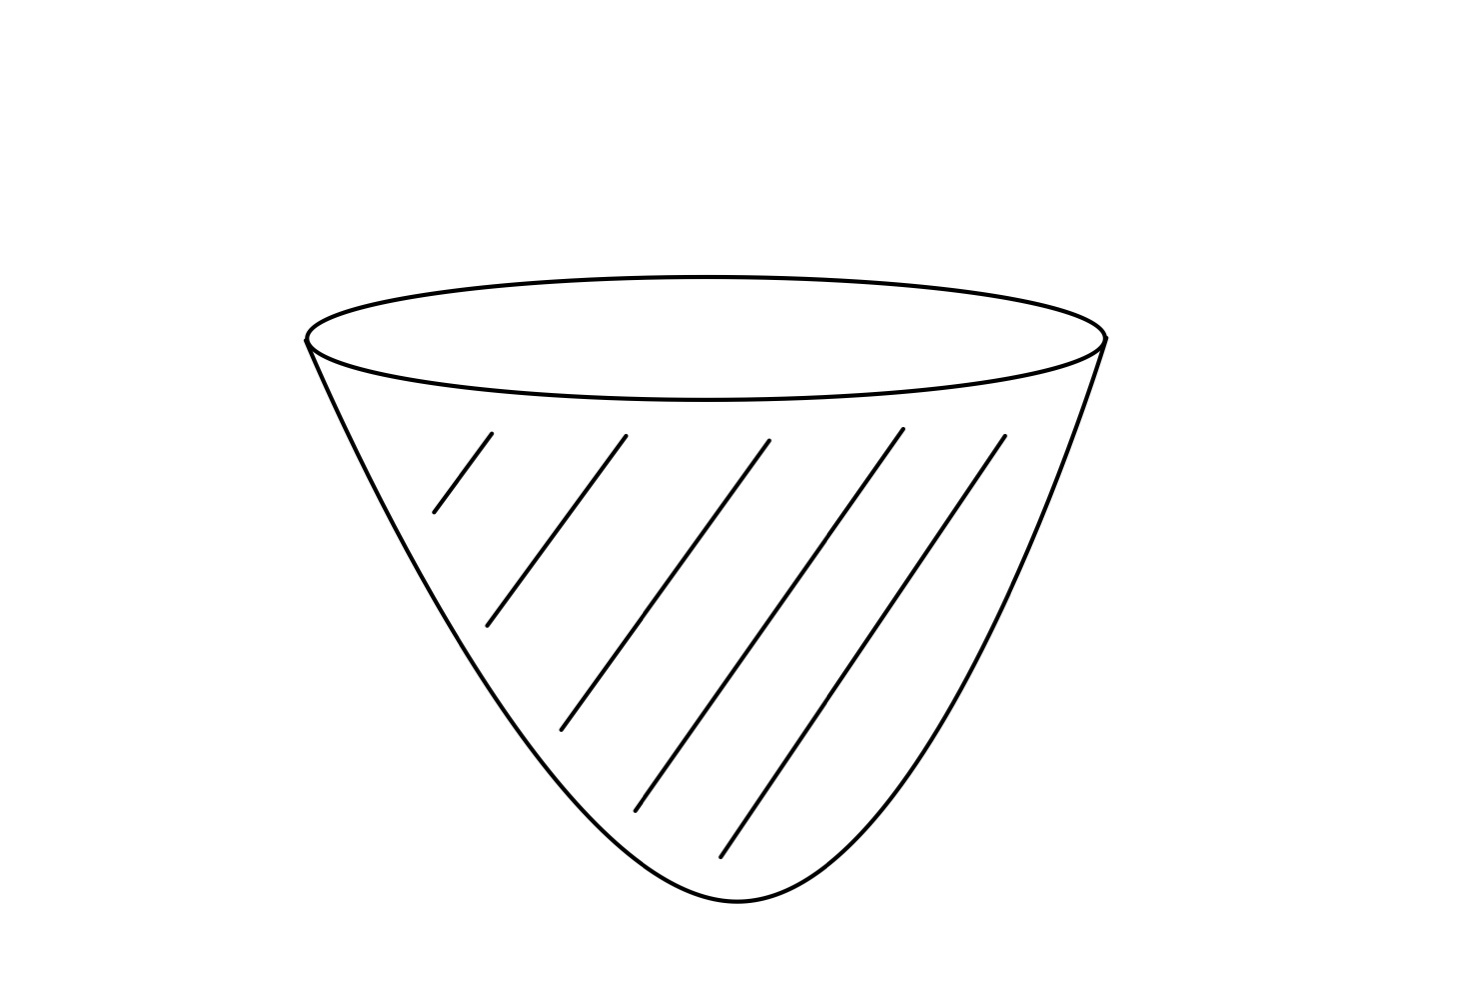
\includegraphics[width = .4\linewidth]{Images_Lect1/2disc.jpeg}
    \caption{0 handle}
    \label{fig:0handleT}
\end{figure}

Since a 0-cell is just $D^{2}$, it's boundary is $S^{1}$, which we can see as the preimage $z\in (a,b)$. The question becomes, \textit{how can we cross the point b?} The answer in this case is by attaching a 1 handle! This is illustrated below in Figure \ref{fig:1handleT}. Similarly, to cross the point c, we again attach a 1-handle (Figure \ref{fig:1handleT2}).
\begin{figure}[h]
    \centering
    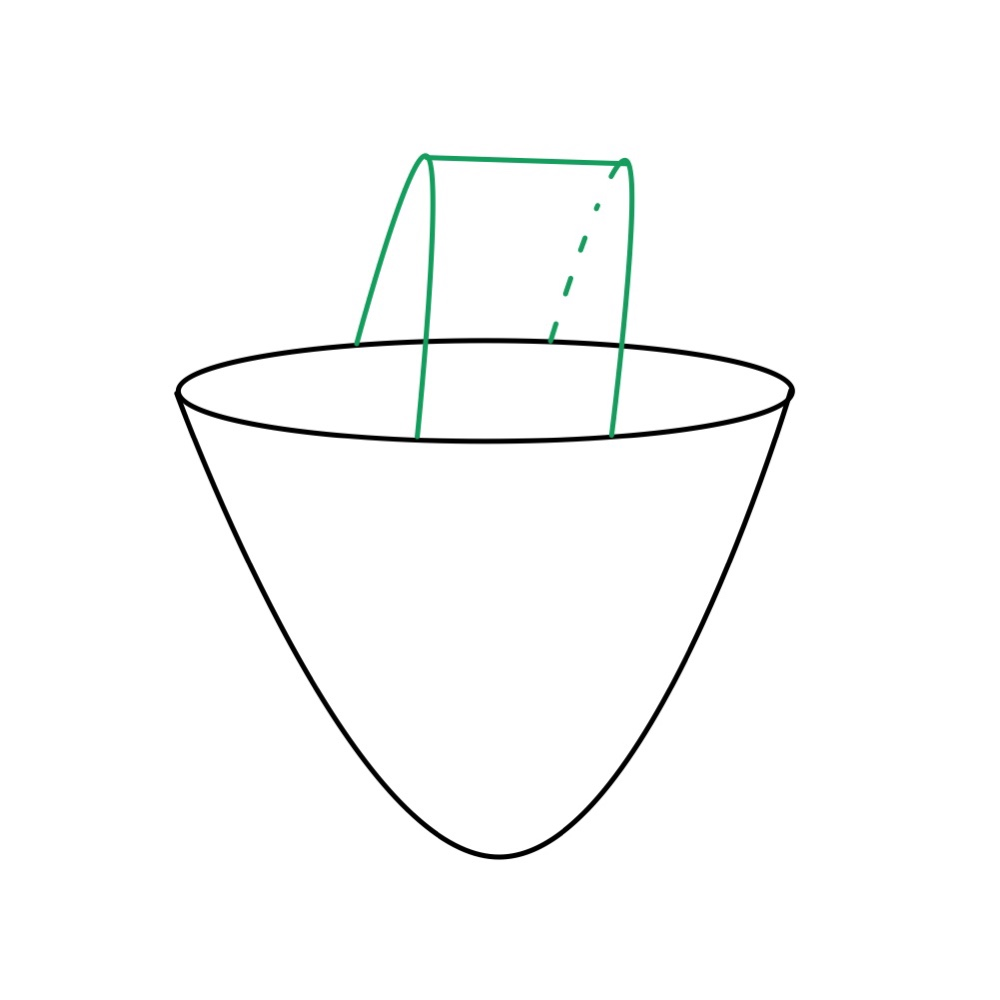
\includegraphics[width = .3\linewidth]{Images_Lect1/1handle.jpeg}
    \caption{Attaching the first 1 handle}
    \label{fig:1handleT}
\end{figure}
\begin{figure}[h]
    \centering
    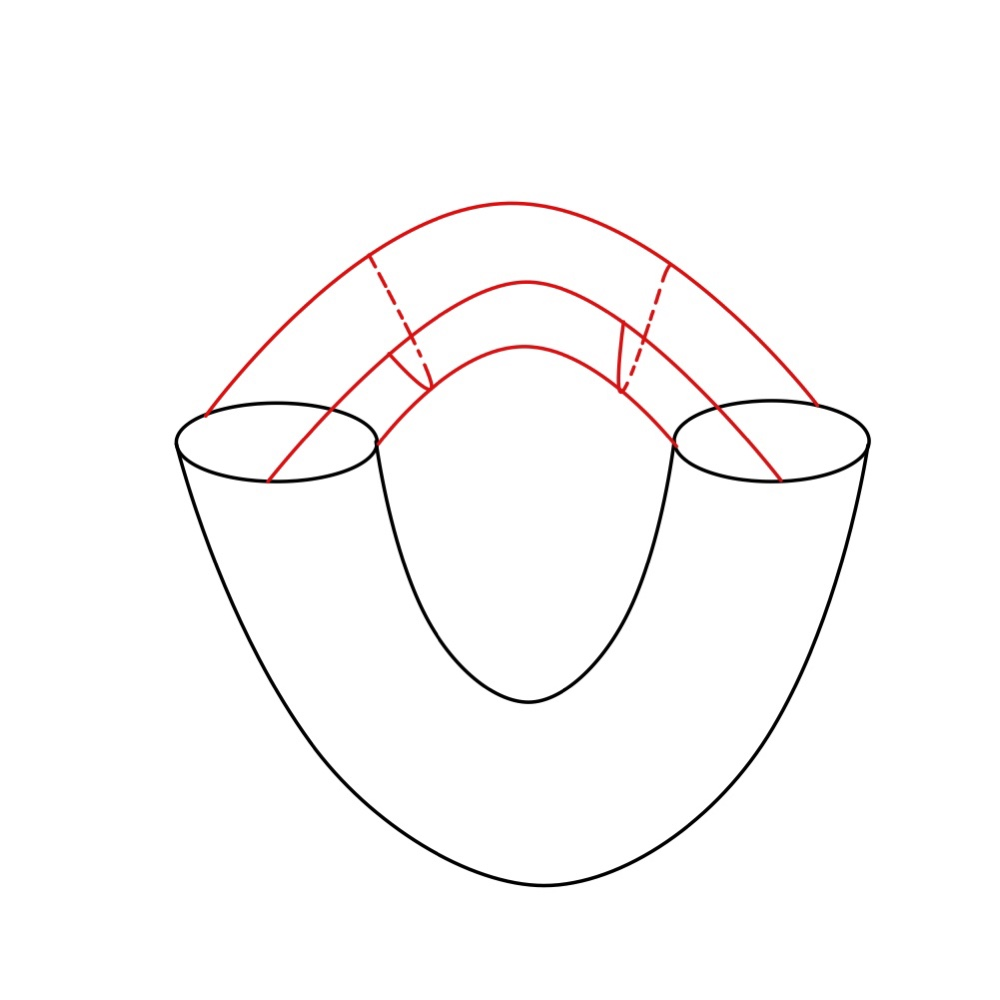
\includegraphics[width = .3\linewidth]{Images_Lect1/1handle2.jpeg}
    \caption{Attaching the second 1 handle}
    \label{fig:1handleT2}
\end{figure}Then finally, we cap off with a 2-handle to complete the picture.
\end{example}
\begin{remark}
As we will see, there is a canonical way to smooth the corners so that our topological space admits a smooth structure.
\end{remark}

The previous two examples illustrates an important idea. The two manifolds $S^{2}$ and $T^{2}$ can be build by attaching handles together. This is so important, we give it a name.
\begin{definition}
Let $M$ be a closed manifold. Then $M$ has a \textbf{handle decomposition} if $M$ is diffeomorphic to a quotient space $X$ of the form
\[
h_{0}\cup_{\phi_{1}}h_{1}\cup_{\phi_{2}}h_{2}...\cup_{\phi_{m}}h_{m}
\]
where $h_{i}$ represent some $k_{i}$ handle with attaching map $\phi_{i}$, $h_{0}$ and $h_{m}$ are a 0 and $n$ handle respectively.
\end{definition}
Now this leads to 3 immediate questions. First, does every closed smooth manifold admit a handlebody decomposition? Second, how many, and how unique are these decompositions, i.e., how are they related? The answer to these questions precipitates us into the next section.

\subsection{Morse Functions and Cobordisms: an introduction.}
Notice in the $S^{2}$ and $T^{2}$ examples, the points where we attached the handles corresponded to the critical points of the projection map. This is no accident and is the main reason why Morse theory is used to study finite dimensional spaces. \textbf{Fact} There is a one to one correspondence between handle decompositions of a manifold and \textit{nice} functions. These nice functions are called Morse functions. So let us give some definitions as to define what exactly a Morse function is.

\begin{definition}
Let $M$ be a smooth manifold and let $f:M\rightarrow \RR$ be a smooth function. A point $p\in M$ is called a \textbf{critical point} if the linear map, $df_{p}:T_{p}M\rightarrow \RR$ is the zero map. Equivalently, if there exist a coordinate system around $p$ such that 
\[
\frac{\partial f}{\partial x_{i}}(p) =0 ~ \text{ for all }~1\leq i \leq n
\]
The value $c\in \RR$ is called a \textbf{critical value} if $f^{-1}(c)$ contains at least on critical point. A critical point, $p$, is called \textbf{non-degenerate} if there exist some coordinate system around $p$ such that 
\[
det\bigg( \frac{\partial^{2} f}{\partial x_{i}{\partial x_{j}}}(p)\bigg)\neq 0
\]
\end{definition}
